
The luminometer data corresponding to the $\mu$-scans is selected by applying selections on the time stamps.
The selections remove luminosity values when the LHC beam conditions are in transition and cause comparisons across luminometers to fail.
The time selections are best determined from one of the luminometers read by the BRIL-DAQ as the temporal granularity has ``nibble'' resolution ($\sim$2s), while the PCC luminosity values are determined every lumi section ($\sim$23s).

Figure~\ref{fig:lumivstime} shows the luminosity vs. time for the HFOC luminometer and the transition time stamps that were determined from these data.
The absolute time stamp values in seconds are the following:
\begin{itemize}
\item Fill 6847 : 1530010610, 1530010615, 1530010670, 1530010721, 1530010772, 1530010824, 1530010875, 1530010926, 1530010978, 1530011031, 1530011082, 1530011133, 1530011184, 1530011235, 1530011287, 1530011339, 1530011393, 1530011441, 1530011489, 1530011537, 1530011585, 1530011633, 1530011681, 1530011729, 1530011761, 1530011811, 1530011863, 1530011914, 1530011966, 1530012019, 1530012070, 1530012122, 1530012173, 1530012225, 1530012277, 1530012328, 1530011400
\item Fill 7358 : 1540537829, 1540537864, 1540537940, 1540538037, 1540538158, 1540538277, 1540538446, 1540538429
\end{itemize}

All data  within 24 seconds of these transitions times are excluded from the analysis, in the case of PCC the luminosity sections with time stamps in these windows are removed.
The data for luminometers with nibble granualurity (HFOC, PLT, BCM) are then averaged within lumi sections for comparison with PCC. 

The PCC and HFOC luminosity values per lumisection before and after the time selections are shown in Figure~\ref{fig:lumivsls}.


\begin{figure}[t]
  \begin{center}
    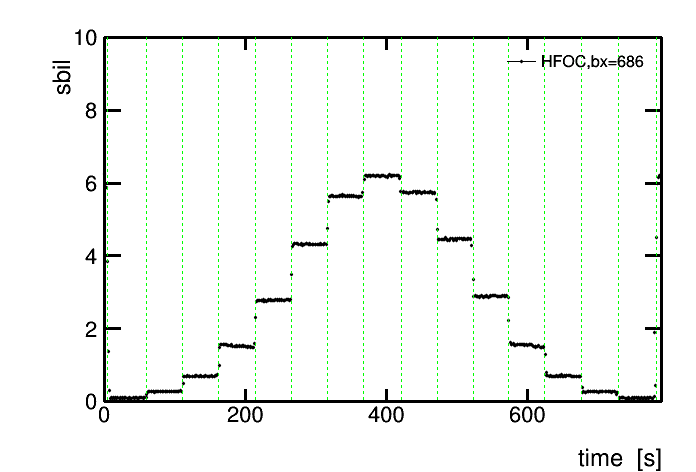
\includegraphics[width=0.47\linewidth]{plots/plot_lumi_vstime_6847.png}
    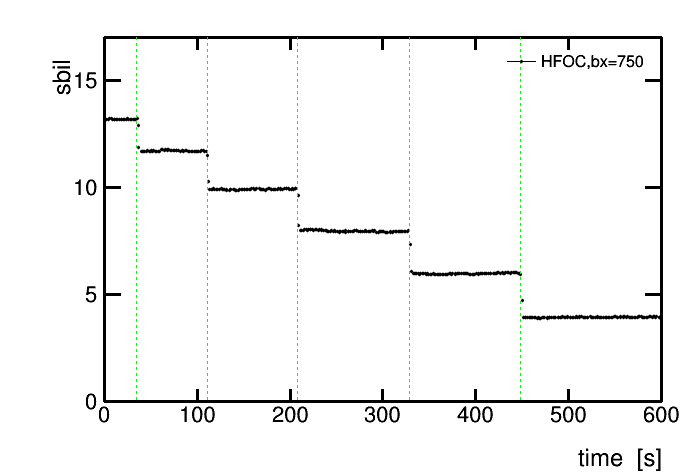
\includegraphics[width=0.47\linewidth]{plots/plot_lumi_vstime_7358.png}
    \caption{
      SBIL data for the HFOC covering the time range of one $\mu$-scan in Fill 6847 (left) and Fill 7358 (right). The vertical lines mark the time stamps determined from this data where the LHC beam parameters are changed.
    \label{fig:lumivstime}
    }
  \end{center}
\end{figure}


\newpage

\begin{figure}[t]
  \begin{center}
    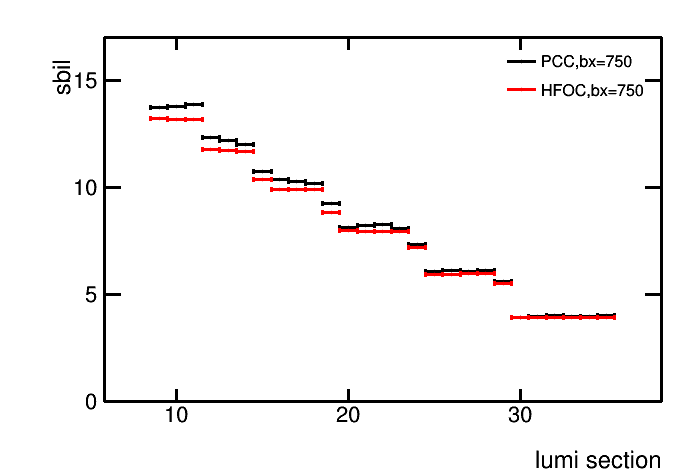
\includegraphics[width=0.6\linewidth]{plots/plot_lumi_vsls_7358_before.png}
    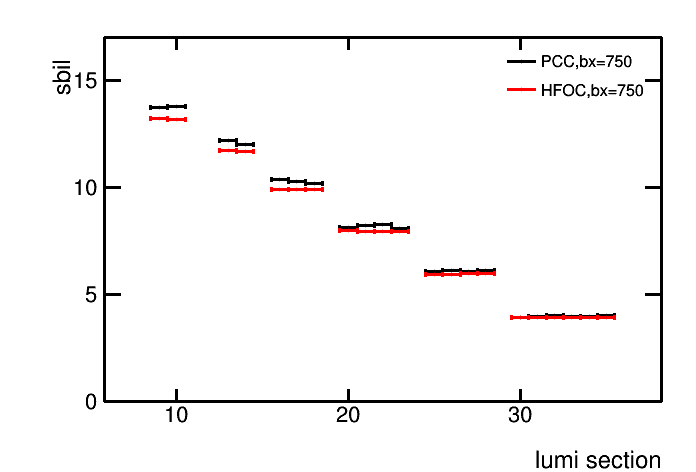
\includegraphics[width=0.6\linewidth]{plots/plot_lumi_vsls_7358_after.png}
    \caption{
    PCC and HFOC single bunch instantenous luminosity (SBIL) after applying afterglow corrections for one bunch crossing in Fill 7358, before (top) and after (bottom) applying the time selections.
    \label{fig:lumivsls}
    }
  \end{center}
\end{figure}
